\subsection{gnuplot}

\begin{frame}[fragile]{convert}
  \begin{itemize}
    \pause \item plot images, graphs, histogram
    \pause \item script to describe how datas are displayed
    \pause \item one or more file containing the datas to display
  \end{itemize}
\end{frame}

\begin{frame}[fragile]{convert}
  \begin{exampleblock}{Gnuplot script}
    \begin{lstlisting}[showstringspaces=false,basicstyle=\tiny]
#!/usr/bin/gnuplot
set style data histogram
set style fill solid border
# Give the bars a plain fill pattern, and draw a sloid line around them
set terminal png
# Make x axis labels easier to read
set xtics rotate out
set output "file.png"
plot 'gnup.dat' using 2:xticlabels(1) title "File size"
    \end{lstlisting}
  \end{exampleblock}
\end{frame}

\begin{frame}[fragile]{convert}
  \begin{figure}[!h]
    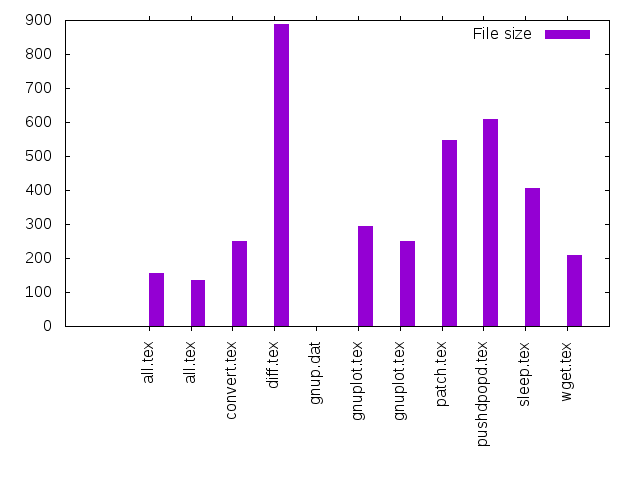
\includegraphics[height=6cm]{img/gnup.png}
  \end{figure}
\end{frame}
